\documentclass[tikz,border=3pt]{standalone}
\usetikzlibrary{arrows.meta,calc}
\begin{document}
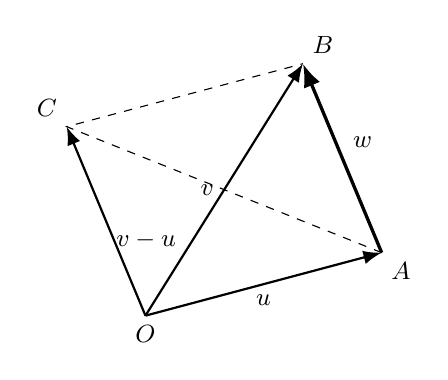
\begin{tikzpicture}[>=Latex, font=\small]
  \coordinate (O) at (0,0);
  \coordinate (A) at (3.0,0.8);
  \coordinate (B) at (2.0,3.2);
  \coordinate (C) at ($(B)-(A)$);

  \draw[dashed] (A) -- (C) -- (B);
  \draw[->, thick] (O) -- (A) node[midway, below] {$u$};
  \draw[->, thick] (O) -- (B) node[midway, left] {$v$};
  \draw[->, thick] (O) -- (C) node[midway, below right] {$v-u$};
  \draw[->, very thick] (A) -- (B) node[midway, above right] {$w$};

  \node[below] at (O) {$O$};
  \node[below right] at (A) {$A$};
  \node[above right] at (B) {$B$};
  \node[above left] at (C) {$C$};
\end{tikzpicture}
\end{document}
